% !TeX spellcheck = en_US
%% abtex2-modelo-relatorio-tecnico.tex, v-1.9.2 laurocesar
%% Copyright 2012-2014 by abnTeX2 group at http://abntex2.googlecode.com/ 
%%
%% This work may be distributed and/or modified under the
%% conditions of the LaTeX Project Public License, either version 1.3
%% of this license or (at your option) any later version.
%% The latest version of this license is in
%%   http://www.latex-project.org/lppl.txt
%% and version 1.3 or later is part of all distributions of LaTeX
%% version 2005/12/01 or later.
%%
%% This work has the LPPL maintenance status `maintained'.
%% 
%% The Current Maintainer of this work is the abnTeX2 team, led
%% by Lauro César Araujo. Further information are available on 
%% http://abntex2.googlecode.com/
%%
%% This work consists of the files abntex2-modelo-relatorio-tecnico.tex,
%% abntex2-modelo-include-comandos and abntex2-modelo-references.bib
%%

% ------------------------------------------------------------------------
% ------------------------------------------------------------------------
% abnTeX2: Modelo de Relatório Técnico/Acadêmico em conformidade com 
% ABNT NBR 10719:2011 Informação e documentação - Relatório técnico e/ou
% científico - Apresentação
% ------------------------------------------------------------------------ 
% ------------------------------------------------------------------------

\documentclass[
	% -- opções da classe memoir --
	12pt,				% tamanho da fonte
	openright,			% capítulos começam em pág ímpar (insere página vazia caso preciso)
	oneside,			% para impressão em verso e anverso. Oposto a oneside
	a4paper,			% tamanho do papel. 
	% -- opções da classe abntex2 --
	%chapter=TITLE,		% títulos de capítulos convertidos em letras maiúsculas
	%section=TITLE,		% títulos de seções convertidos em letras maiúsculas
	%subsection=TITLE,	% títulos de subseções convertidos em letras maiúsculas
	%subsubsection=TITLE,% títulos de subsubseções convertidos em letras maiúsculas
	% -- opções do pacote babel --
	english,			% idioma adicional para hifenização
	french,				% idioma adicional para hifenização
	spanish,			% idioma adicional para hifenização
	brazil,				% o último idioma é o principal do documento
	]{abntex2}


% ---
% PACOTES
% ---

% ---
% Pacotes fundamentais 
% ---
\usepackage{lmodern}			% Usa a fonte Latin Modern
\usepackage[T1]{fontenc}		% Selecao de codigos de fonte.
\usepackage[utf8]{inputenc}		% Codificacao do documento (conversão automática dos acentos)
\usepackage{indentfirst}		% Indenta o primeiro parágrafo de cada seção.
\usepackage{color}				% Controle das cores
\usepackage{graphicx}			% Inclusão de gráficos
\usepackage{microtype} 			% para melhorias de justificação
\usepackage{amssymb}
\usepackage[boxruled, linesnumbered, portuguese]{algorithm2e}
\usepackage{alltt}
% ---

% ---
% Pacotes adicionais, usados no anexo do modelo de folha de identificação
% ---
\usepackage{multicol}
\usepackage{multirow}
% ---
	
% ---
% Pacotes adicionais, usados apenas no âmbito do Modelo Canônico do abnteX2
% ---
\usepackage{lipsum}				% para geração de dummy text
% ---

% ---
% Pacotes de citações
% ---
\usepackage[brazilian,hyperpageref]{backref}	 % Paginas com as citações na bibl
\usepackage[alf]{abntex2cite}	% Citações padrão ABNT

% --- 
% CONFIGURAÇÕES DE PACOTES
% --- 

% ---
% Configurações do pacote backref
% Usado sem a opção hyperpageref de backref
\renewcommand{\backrefpagesname}{Citado na(s) página(s):~}
% Texto padrão antes do número das páginas
\renewcommand{\backref}{}
% Define os textos da citação
\renewcommand*{\backrefalt}[4]{
	\ifcase #1 %
		Nenhuma citação no texto.%
	\or
		Citado na página #2.%
	\else
		Citado #1 vezes nas páginas #2.%
	\fi}%
% ---

% ---
% Informações de dados para CAPA e FOLHA DE ROSTO
% ---
\titulo{Matrizes Ortogonais e o \\Problema de Quadrados Mínimos}
\autor{Florence Alyssa Sakuma Shibata \and Shayenne da Luz Moura}
\local{São Paulo}
\data{2014}
\instituicao{%
  Universidade de São Paulo -- USP
  \par
  Instituto de Matemática e Estatística
  \par
  Bacharelado em Ciência da Computação}
\tipotrabalho{Relatório técnico}
% O preambulo deve conter o tipo do trabalho, o objetivo, 
% o nome da instituição e a área de concentração 
\preambulo{Relatório dos resultados dos testes do segundo trabalho menor.}
% ---

% ---
% Configurações de aparência do PDF final

% alterando o aspecto da cor azul
\definecolor{blue}{RGB}{41,5,195}

% informações do PDF
\makeatletter
\hypersetup{
     	%pagebackref=true,
		pdftitle={\@title}, 
		pdfauthor={\@author},
    	pdfsubject={\imprimirpreambulo},
	    pdfcreator={LaTeX with abnTeX2},
		pdfkeywords={abnt}{latex}{abntex}{abntex2}{relatório técnico}, 
		colorlinks=true,       		% false: boxed links; true: colored links
    	linkcolor=blue,          	% color of internal links
    	citecolor=blue,        		% color of links to bibliography
    	filecolor=magenta,      		% color of file links
		urlcolor=blue,
		bookmarksdepth=4
}
\makeatother
% --- 

% --- 
% Espaçamentos entre linhas e parágrafos 
% --- 

% O tamanho do parágrafo é dado por:
\setlength{\parindent}{1.3cm}

% Controle do espaçamento entre um parágrafo e outro:
\setlength{\parskip}{0.2cm}  % tente também \onelineskip

% ---
%% compila o indice
%% ---
\makeindex
% ---

% ----
% Início do documento
% ----
\begin{document}

% Retira espaço extra obsoleto entre as frases.
\frenchspacing 

% ----------------------------------------------------------
% ELEMENTOS PRÉ-TEXTUAIS
% ----------------------------------------------------------
\pretextual

% ---
% Capa
% ---
\imprimircapa
% ---

% ---
% Folha de rosto
% (o * indica que haverá a ficha bibliográfica)
% ---
%\imprimirfolhaderosto*
% ---


% ---
% RESUMO
% ---

% resumo na língua vernácula (obrigatório)
\setlength{\absparsep}{18pt} % ajusta o espaçamento dos parágrafos do resumo
\begin{resumo}
Este relatório trata do desenvolvimento do algoritmo da decomposiçao QR
 por refletores, com implementacao do posto incompleto e tambem de seu uso
 para resolucao de ajuste de curvas pelo metodo dos minimos quadrados.Por fim, todos os resultados foram condizentes com 
o esperado.

 \noindent
 \textbf{Palavras-chaves}: QR. problema quadrados mínimos. resolução de sistemas lineares.
\end{resumo}
% ---

%% ---
%% inserir lista de ilustrações
%% ---
%\pdfbookmark[0]{\listfigurename}{lof}
%\listoffigures*
%\cleardoublepage
%% ---
%
%% ---
%% inserir lista de tabelas
%% ---
%\pdfbookmark[0]{\listtablename}{lot}
%\listoftables*
%\cleardoublepage
%% ---
%
%% ---
%% inserir lista de abreviaturas e siglas
%% ---
%\begin{siglas}
%  \item[ABNT] Associação Brasileira de Normas Técnicas
%  \item[abnTeX] ABsurdas Normas para TeX
%\end{siglas}
%% ---
%
%% ---
%% inserir lista de símbolos
%% ---
%\begin{simbolos}
%  \item[$ \Gamma $] Letra grega Gama
%  \item[$ \Lambda $] Lambda
%  \item[$ \zeta $] Letra grega minúscula zeta
%  \item[$ \in $] Pertence
%\end{simbolos}
%% ---
%
%% ---
% inserir o sumario
% ---
\pdfbookmark[0]{\contentsname}{toc}
\tableofcontents*
\cleardoublepage
%% ---
%
%
%% ----------------------------------------------------------
%% ELEMENTOS TEXTUAIS
%% ----------------------------------------------------------
%\textual

% ----------------------------------------------------------
% Introdução
% ----------------------------------------------------------
\chapter*[Introdução]{Introdução}
\addcontentsline{toc}{chapter}{Introdução}

Em investigações científicas é comum buscar relações entre dados pontuais. Normalmente tem-se 
muitos pontos coletados em experimento e há sempre uma razão teórica para acreditar 
que esses pontos são aproximados por uma função.

Como é praticamente impossível que uma função atravesse exatamente todos os pontos de dados
é interessante encontrar uma função que tenha a uma distância aceitável, ou seja, que
possua o menor desvio médio possível.



Encontrar essa função é, na realidade, encontrar a solução de um sistema linear sobredeterminado,
isto é, um sistema com mais equações que incógnitas, $Ax = b$, onde 
$A \in  \mathbb{R}^{n \times m}, n \ge m \ e \ b \in \mathbb{R}^n$. Sendo $A$ a matriz que define o sistema,
$n$ o número de equações, $m$ o número de incógnitas e $b$ os dados do problema. 

Para analisar quão boa é essa aproximação utilizou-se o método dos quadrados mínimos. Para tal, deve-se encontrar a função que minimiza as distâncias entre a solução calculada e os valores observados. 

Neste caso, o problema consiste em encontrar $x \in \mathbb{R}^n$ para o qual $\|r\|_2$ é minimizada, onde $r =  b-Ax$ é o vetor de 
resíduos. 

Para resolver esse problema, utilizou-se o conceito de matriz ortogonal, que é uma matriz quadrada cuja
inversa coincide com sua transposta, por esta possuir número de condição igual a 1, isto é, é bem condicionada.
Matrizes ortogonais nos permitem realizar operações com o sistema $Ax=b$ sem perder a precisão de sua solução.







% ----------------------------------------------------------
% PARTE - preparação da pesquisa
% ----------------------------------------------------------
\part{Teoria do algoritmo}

% ----------------------------------------------------------
% Capitulo com exemplos de comandos inseridos de arquivo externo 
% ----------------------------------------------------------

\chapter{Método QR}

	\section{Decomposição da matriz A}
	Se A for uma matriz não-singular então é possível decompô-la em um produto de matrizes 
	$QR$, onde $Q$ é ortogonal e $R$ é uma matriz triangular superior de diagonal não-nula. Esta decomposição é única e sempre existe.
	
	Para obter essa decomposição deve-se encontrar uma sequência de $Q_i ^T$, $i~ =~ 1,...,m$ onde m é o número de colunas do sistema, sendo que cada uma dessas $Q_i^T$ transforma cada $i$-ésima coluna em zeros abaixo da $i$-ésima posição, formando assim a matriz triangular superior $R$.\cite{sawp} Tendo assim que
	
	\[Q_{n-1} ^TQ_{n-2} ^T \ldots Q_{1} ^T A = R\]
	
	Como cada $Q_i ^T$ é ortogonal, temos $A = QR$, onde \[Q = [Q_{n-1} ^T Q_{n-2} ^T \ldots Q_{1} ^T]^T \]
	\section{Cálculo do vetor x}
	Para resolver um sistema $Ax=b$ podemos decompor a matriz $A$ em termos de $Q$ e $R$ como \[ A = Q{R \brack 0}\] com a matriz $Q$ sendo quadrada de dimensão $n\times n$ e $R$ triangular-superior de dimensão~ $n\times m$.
	A equação toma a forma \[Q^Tx = b\] que pode ser escrito como \[Rx=Q^Tb\]
	Pode-se então separar a solução em dois passos:
	\begin{enumerate}
	\item Calcular $y = Q^Tb$
	\item Resolver o sistema $Rx = y$
	\end{enumerate}
	
	No desenvolvimento do algoritmo não se calculou explicitamente as matrizes $Q$ e $R$ para aumentar sua eficiência. A forma com que os valores necessários para o cálculo da solução são armazenados e utilizados está descrito no algoritmo para decomposição $QR$.
	
	\section{Reutilização do QR para qualquer b}
	Uma vez calculada a decomposição $QR$ de uma matriz $A$, basta realizar os passos anteriores e obter novas soluções variando apenas os dados de $b$.

	\begin{enumerate}
	\item Calcular $y = Q^Tb$
	\item Resolver o sistema $Rx = y$
	\end{enumerate}
	
	Dessa forma, pode-se reaproveitar todo o processamento das matrizes $QR$ e reduzir o tempo de resolução do algoritmo
	a apenas o cálculo de um produto matriz vetor e uma solução de matriz triangular superior.
	Caso não houvesse esse reaproveitamento, a cada novo vetor de dados $b$ para uma mesma matriz $A$ seriam necessários todos os cálculos para decomposição, o que levaria muito processamento desnecessário.
\chapter{Método dos Quadrados Mínimos}

	\section{Descrição}
	O Método dos Quadrados Mínimos é uma técnica de otimização matemática que procura encontrar o melhor ajuste para um 
	conjunto de dados tentando minimizar a soma dos quadrados das diferenças entre o valor estimado e os dados observados.
	Tais diferenças são chamadas resíduos.
	
	
	Consiste em um estimador que minimiza a soma dos quadrados dos resíduos, de forma a maximizar o grau de ajuste do modelo aos dados observados.\cite{wikipedia}
	
	\section{Ordem do algoritmo}
	Calculando a ordem do algoritmo, temos:
	
	Passo 1: ordem $nm$;

	Passo 2: ordem $[(nm)+(m-1)+(m-2)+\ldots +1] \approx nm + m^2$;
	
	Passo 3: ordem $nm$;
	
	Passo 4: ordem $n + (n-1) + \ldots + 1 \approx n^2$;
	
	Passo 5: ordem $3nm + 3(n-1)(m-1) + \ldots + 3 \approx nm^2$;
	
	No total: $\approx m^2+n^2+3nm+m^2 n$.



\chapter{Algoritmo para decomposição QR}


A decomposição da matriz $A \in R^{n\times m}$
 em $QR$, $Q \in R^{n\times n}$, $R \in R^{n\times m}$, $n > m$ segue os seguintes passos:
\newline


1) Determinar o elemento de maior valor $max$ da matriz $A$ e determinar $Â = \frac{1}{max}A$;

Loop ($i = 0 ... m$)

2) Calcular a norma das colunas da submatriz $Â_{(n-i)\times (m-i)}$ e armazenar no vetor sigma;

3) Permutar a coluna $i$ com a que possuir maior norma em sigma (busca nos índices $k = i \ldots m$). Caso a maior norma seja menor que epsilon parar;

4) Encontrar $u, u^T e \gamma $ para determinar $Q= I - \gamma u u^T$;

5) Calcular $QÂ_i$ e armazenar $u$.
\newline


O passo 1 tem por objetivo evitar overflow nos cálculos das normas, pois $\forall a_{ij} \le |1|$.

A iteração sobre o passo 2 e 3 'empurram’ possíveis pivôs nulos para a matriz, no caso de $A$ possuir posto incompleto. Para o recálculo das normas basta extrair os elementos de cada coluna da linha anterior a partir da iteração $i = 1 \ldots r$ ($r$ = posto de $A$).

No passo 5, é possível calculá-lo de forma econômica processando  $QA= A - u((\gamma  u^T)A)$

Como as linhas da coluna $i$ serão zeradas, nestas posições são armazenadas o vetor u.



\part{Testes}

\chapter{Testes de eficiência do algoritmo}
Aqui estão descritos os testes do algoritmo de acordo com a matriz $A$ dada.

\section{Posto completo}
A entrada do algoritmo recebeu uma matriz $A$ com posto completo para realizar
o cálculo da solução e seu resíduo em quadrados mínimos e o vetor $b$.

Para a construcao do suposto polinômio de grau 5, foi construida a matriz $Ax = b$
onde:

\[
A =	\left(
\begin{array}{ccccc} 
1&	x_1^1&	x_1^2&	x_1^3&	x_1^4\\
1&	x_2^1&	x_2^2&	x_2^3&	x_2^4\\
&&\ldots\\
1&	x_k^1&	x_k^2&	x_k^3&	x_k^4\\
\end{array}
\right)
b =   
\left(
\begin{array}{c}
y_1\\
y_2\\
\ldots\\
y_{k-1}\\
y_k 
\end{array}    
\right)
\]

Comparando-o ao polinômio original e verificando se os coeficientes 
são razoavelmente próximos do original.


Para a construção do polinômio de grau 4 foi construida a matriz $Ax = b$ de forma
semelhante ao de grau 5:
\[A =	
\left(
\begin{array}{cccc}
1 &	x_1^1 &	x_1^2 &	x_1^3\\
1 &	x_2^1 &	x_2^2 &	x_2^3\\
&&\dots          \\
1 &	x_k^1 &	x_k^2 &	x_k^3\\
\end{array} 
\right)
b =  
\left(
\begin{array}{c}
y_1\\
y_2\\
\ldots\\
y_{k-1}\\
y_k\\ 
\end{array}   
\right)
\]
A mesma construção foi utilizada para polinômios de grau 3 e 2.


\section{Posto incompleto}

A entrada do algoritmo recebeu uma matriz A com posto imcompleto para realizar
o cálculo da solução e seu resíduo em quadrados mínimos.


\chapter{Efeitos da perturbação em diferentes funções}
Os dados raramente são exatos ao serem representados no computador, até mesmo na 
coleta destes podem haver erros de aproximação e medida que podem interferir no
resultado esperado do sistema.
Agora será descrito o que ocorre ao perturbar os valores das entradas e 
comparar as soluções anteriores e o quanto isso influencia no cálculo das 
soluções encontradas.

\section{Diminuir ou aumentar o grau do polinômio}
Soluções com diferentes graus polinomiais podem aproximar de forma diferente
os dados do problema.
Os graus em que foram testados o algoritmo foram 2, 3, 4 e 5.
A partir destas foram feitas perturbações nos dados para comparar os resultados.

\section{Nos valores de b}
Os dados do vetor de entrada b foram perturbados em 15\% e foram mantidos os
valores de A.
A compararação dos resultados foram feitas de acordo com o grau do polinômio. 
\section{Nos valores de A e b}

Os dados do vetor de entrada de A e b foram perturbados em 15\%.
A compararação dos resultados foram feitas de acordo com o grau do polinômio.




% ----------------------------------------------------------
% Parte de revisãod e literatura
% ----------------------------------------------------------
\part{Resultados}

% ---
% Capitulo de revisão de literatura
% ---


\chapter{Resolução de sistema com posto incompleto}
Para o teste do posto incompleto, foi gerado $Ax = b$ onde:


\[
A =
\left(
\begin{array}{ccc}
	1.0000000 & 0.0000000 & 1.0000000\\
	2.0000000 & 5.0000000 & 2.0000000\\
	-1.0000000 & -5.0000000 & -1.0000000\\
	-1.0000000 & 0.0000000 & -1.0000000\\
\end{array}
\right)
\]
\[
b =
\left(
\begin{array}{c}
10.000  \\
45.000  \\
-35.000  \\
-10.000  \\
\end{array}\right)    
\]
com valores pré-determinados\[ x = 
\left(
\begin{array}{c}
6\\
5\\
4\\
\end{array}
\right)\]

Note que a terceira e a quarta linha sao combinações lineares da primeira e segunda linha.

Enviando este arquivo para o programa, temos como resultado:
\(x_0 = 10.00000 $e$ x_1 = 5.00000 \) com resíduo = 16.44817 .

Tem-se para as soluções geradas do programa, o mesmo resultado $b$. É razoavel, 
uma vez que a matriz $A$ e singular. 


\chapter{Resolução de sistema com posto completo e problema dos quadrados mínimos}
Inicialmente foi tomado o polinômio $x^5-7x^4+5x^3-3x^2+2x-1$ e sorteados
70 pontos para servirem como  dados de entrada e foram calculadas as funções que
melhor aproximariam esses pontos.
As funções soluções foram encontradas em diferentes graus. 

Após, os dados foram perturbados em 15\% e foram calculadas novas
soluções. Estas funçoes e suas características de aproximação estão descritas 
a seguir.

\section{Dados iniciais}
Os pontos sorteados e a função caracterizadas pelo polinômio \[x^5~-~7x^4~+~5x^3~-~3x^2~+~2x~-~1\]
estão plotados abaixo.

\begin{figure}[h]
\centering
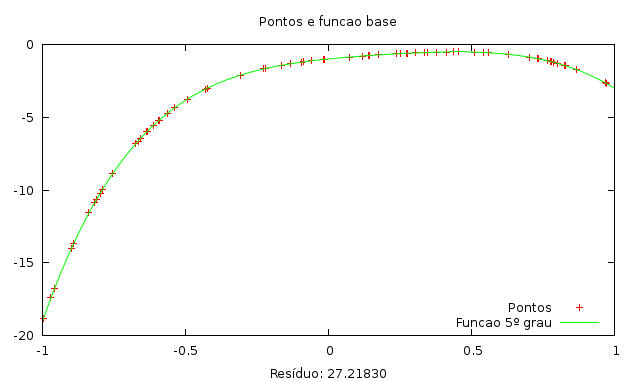
\includegraphics[scale=0.7]{funcbase}
\end{figure}

Os pontos foram usados para buscar funções que os atravessassem reduzindo o resíduo.
A partir dessas soluções, os dados foram perturbados e suas novas funções calculadas.



\newpage
\section{Solução 2º grau}

Ao buscar uma função de grau 2 para aproximar os pontos encontrou-se os seguintes 
coeficientes:

\(x_0 = -3.74052 ~$e$~  x_1 = 5.87079 \)

\begin{figure}[h]
\centering
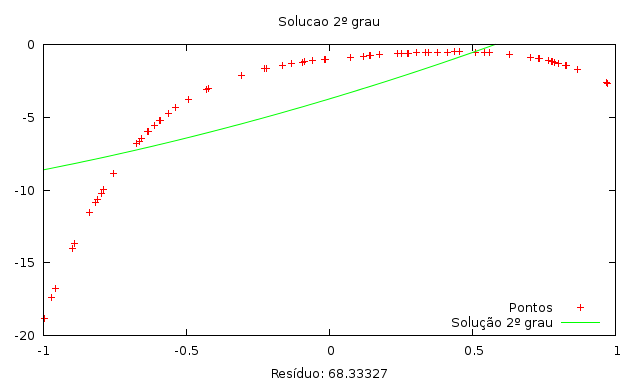
\includegraphics[scale=0.7]{sol2grau}
\end{figure}

Ao perturbar os dados de entrada em 15\%, o programa calculou as funções 
com resíduos 80.79981 para perturbação em $b$ e 88.55303 para perturbação em $A$ e $b$.

\begin{figure}[h]
\centering
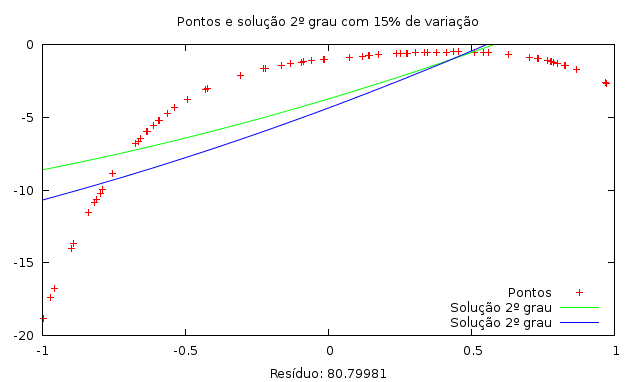
\includegraphics[scale=0.7]{sol2grau_var}
\end{figure}


\newpage
\section{Solução 3º grau}

Ao buscar uma função mônica de grau 3 para aproximar os pontos encontrou-se os seguintes 
coeficientes:

\(x_0 = -0.39367  ,~  x_1 = 5.45203  ~$e$~ x_2 = -9.03908 \)

\begin{figure}[h]
\centering
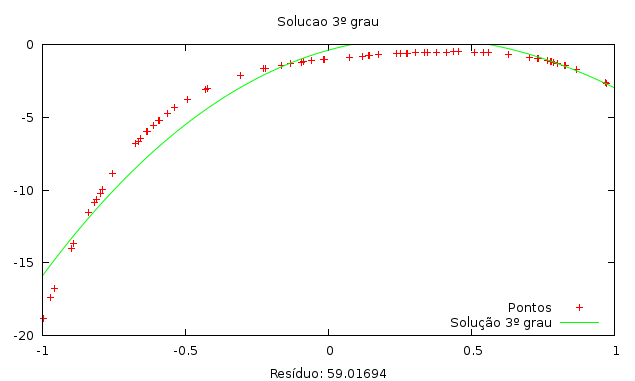
\includegraphics[scale=0.7]{sol3grau}
\end{figure}

Ao perturbar os dados de entrada em 15\%, o programa calculou as funções 
com resíduos 69.37743  para perturbação em $b$ e 68.57657 para perturbação em $A$ e $b$.
\begin{figure}[h]
\centering
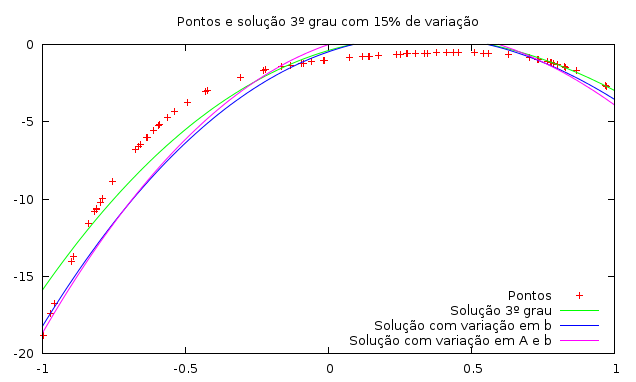
\includegraphics[scale=0.7]{sol3grau_var}
\end{figure}

\newpage
\section{Solução 4º grau}

Ao buscar uma função mônica de grau 4 para aproximar os pontos encontrou-se os seguintes 
coeficientes:
\(x_0 = -0.34728 ,~  x_1 = 1.25949,~ x_2 =  -8.95480 ~$e$~ x_3 = 6.95427 \)

\begin{figure}[h]
\centering
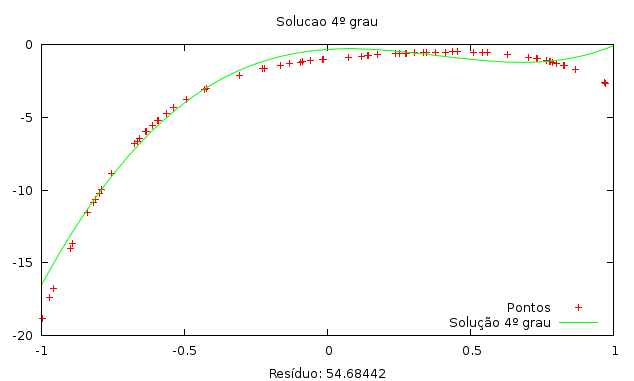
\includegraphics[scale=0.7]{sol4grau}
\end{figure}
Ao perturbar os dados de entrada em 15\%, o programa calculou as funções 
com resíduos 64.67217 para perturbação em $b$ e 56.54760  para perturbação em $A$ e $b$.
\begin{figure}[h]
\centering
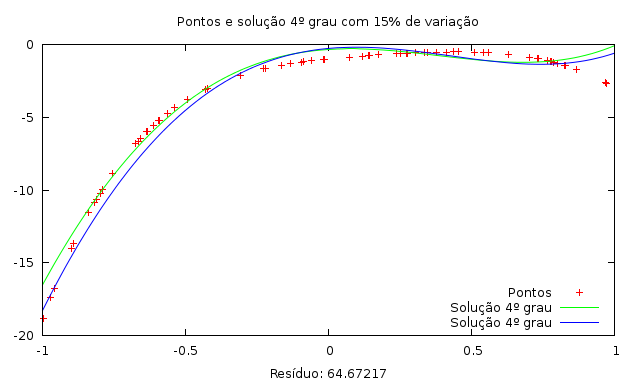
\includegraphics[scale=0.7]{sol4grau_var}
\end{figure}

\newpage
\section{Solução 5º grau}

Ao buscar uma função mônica de grau 5 para aproximar os pontos encontrou-se os seguintes 
coeficientes:

\(x_0 = -0.99223,~    x_1 = 1.73653,~x_2 = -2.98373,~ x_3 = 6.13233 ~$e$~ x_4 =  -7.05190 \)

\begin{figure}[h]
\centering
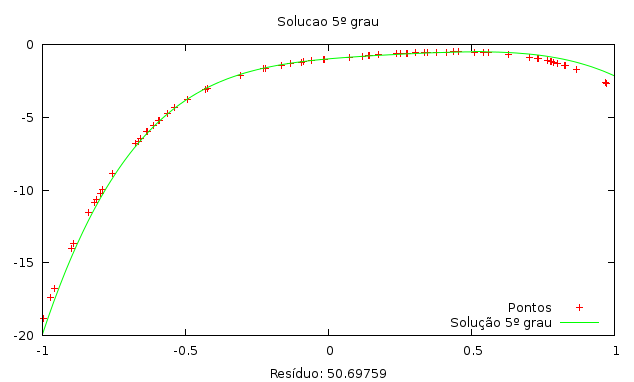
\includegraphics[scale=0.7]{sol5grau}
\end{figure}
Ao perturbar os dados de entrada em 15\%, o programa calculou as funções 
com resíduos 61.44919  para perturbação em $b$ e 47.96817 para perturbação em $A$ e $b$.
\begin{figure}[h]
\centering
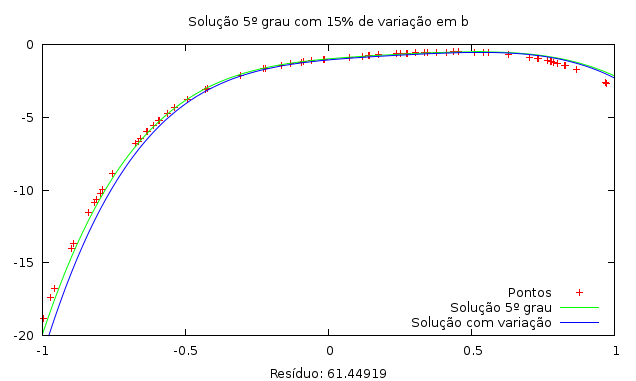
\includegraphics[scale=0.7]{sol5grau_var}
\end{figure}


% ---
% Finaliza a parte no bookmark do PDF
% para que se inicie o bookmark na raiz
% e adiciona espaço de parte no Sumário
% ---
\phantompart

% ---
% Conclusão
% ---
\chapter*[Conclusão]{Conclusão}
\addcontentsline{toc}{chapter}{Conclusão}

\lipsum[31-33]

% ----------------------------------------------------------
% ELEMENTOS PÓS-TEXTUAIS
% ----------------------------------------------------------
\postextual

% ----------------------------------------------------------
% Referências bibliográficas
% ----------------------------------------------------------
\bibliography{references}

% ----------------------------------------------------------
% Glossário
% ----------------------------------------------------------
%
% Consulte o manual da classe abntex2 para orientações sobre o glossário.
%
%\glossary

% ----------------------------------------------------------
% Apêndices
% ----------------------------------------------------------

% ---
% Inicia os apêndices
% ---
%\begin{apendicesenv}
%
%% Imprime uma página indicando o início dos apêndices
%\partapendices
%
%% ----------------------------------------------------------
%\chapter{Quisque libero justo}
%% ----------------------------------------------------------
%
%\lipsum[50]
%
%% ----------------------------------------------------------
%\chapter{Nullam elementum urna vel imperdiet sodales elit ipsum pharetra ligula
%ac pretium ante justo a nulla curabitur tristique arcu eu metus}
%% ----------------------------------------------------------
%\lipsum[55-57]
%
% \end{apendicesenv}
%% ---
%
%
% ----------------------------------------------------------
% Anexos
% ----------------------------------------------------------

% ---
% Inicia os anexos
% ---
%\begin{anexosenv}
%
%% Imprime uma página indicando o início dos anexos
%\partanexos
%
%% ---
%\chapter{Morbi ultrices rutrum lorem.}
%% ---
%\lipsum[30]
%
%% ---
%\chapter{Cras non urna sed feugiat cum sociis natoque penatibus et magnis dis
%parturient montes nascetur ridiculus mus}
%% ---
%
%\lipsum[31]
%
%% ---
%\chapter{Fusce facilisis lacinia dui}
%% ---
%
%\lipsum[32]
%
%\end{anexosenv}
%%

\end{document}
